\newpage
\section{Auswertung}

\subsection{Quarzkügelchen}
    Für die weitere Auswertung ist es fundamental die Auflösung der aufgenommen Bilder zu kennen.
    Zu diesem Zweck wird die Größe eines Pixels in der CCD-Kamera-Software bestimmt.
    Die Größe der verwendeten Quarzkügelchen ist mit \qty{2,06}{\um} bekannt.
    Befindet sich nun ein Quarzkügelchen im Fokus des Mikroskops bzw. der Falle, wird es mit dem Zeichenwerkzeug markiert, siehe \autoref{fig:Pixelgroesse}.
    \begin{figure}[ht]
        \centering\captionsetup{format=plain}
        \includegraphics[width=0.5\textwidth]{bilder/Pixelgröße.JPG}
        \caption{Markierung eines eingefangenen Quarzkügelchens im Fokus des Mikroskops zur Bestimmung der Größe eines Pixels.}
        \label{fig:Pixelgroesse}
    \end{figure}
    \FloatBarrier
    Nach dem Zählen der Pixel entlang des Durchmessers des gelben Kreises ergibt sich die Pixelgröße zu
    \begin{equation}
        \mathrm{Pixelgröße} = \frac{\SI{2,06}{\um}}{122} \approx \SI{16,9}{\nm} \;.
    \end{equation}

\subsection{Kalibrierung der Spannung der Viersegment-Photodiode}
    Den Quarzkugeln wird NaCl-haltiges Wasser beigemischt.
    Die Kationen schirmen die elektrische Ladung der negativ geladenen Kugel ab, was ein Festkleben an den Wänden der Probenkammer wahrscheinlicher macht.
    Nun ist es möglich Messungen durchzuführen ohne, dass sich die Quarzkugeln bewegen.

    Zur Umrechnung des Spannungssignals der Viersegment-Photodiode in die tatsächliche Position in der Fokusebene des Mikroskops wurde die Optische Pinzette in x- und y-Richtung über eine fixierte Quarzkugel gescannt.
    Dabei wurde das auf der Photodiode gemessene Spannungssignal gegen die Position aufgetragen.
    Dies wurde für mehrere Laserleistungen durchgeführt, hier wird die Vorgehensweise exemplarisch nur für \qty{200}{mA} gezeigt.
    An den in \autoref{fig:PosCal_200mA} zu sehenden S-Kurven zwischen den blauen Linien wurden lineare Regressionen durchgeführt, um die Steigungen zu bestimmen.
    Diese geben die Konversationsfaktoren zwischen Photodiodenspannung und Position an.

    \begin{figure}[ht]
        \centering\captionsetup{format=plain}
        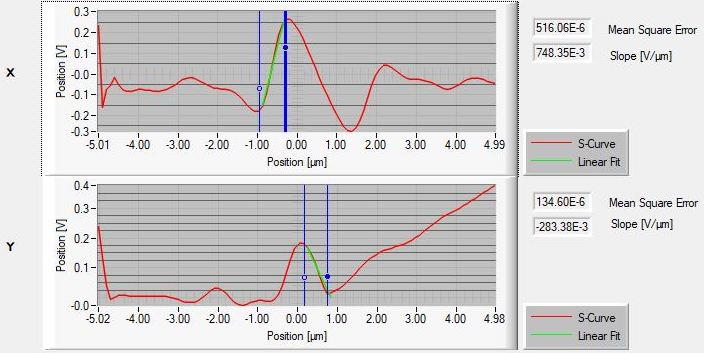
\includegraphics[width=0.6\textwidth]{bilder/PosCal_200mA.JPG}
        \caption{Ein Screenshot aus dem Thorlabs Programm im Menüpunkt \glqq \textit{position calibration} von einem Scan über eine fixierte Quarzkugel. Die Steigung der Flanken wird durch die grüne Gerade gefittet und gibt den Konversationsfaktor zwischen Photodiodenspannung und Position an.}
        \label{fig:PosCal_200mA}
    \end{figure}
    \FloatBarrier
    Trägt man die Konversationsfaktoren für verschiedene Laserleistungen auf, so ist kein deutlicher Trend zu erkennen.
    Es ist jedoch möglich die durchschnittlichen Konsversationsfaktoren für die x- und y-Richtung zu bestimmen:
    \begin{equation*}
        m_{\mathrm{x,konv}} \approx \qty{0,71}{V m^{-1}} \qquad m_{\mathrm{y,konv}} \approx \qty{0,29}{V m^{-1}}
    \end{equation*}
    \begin{figure}[ht]
        \centering\captionsetup{format=plain}
        \includegraphics[width=0.6\textwidth]{plots/Konversionsfaktoren.pdf} \vspace*{-0.5cm}
        \caption{Hier sind die Konversationsfaktoren für verschiedene Laserleistungen aufgetragen.}
        \label{fig:Konversionsfaktoren}
    \end{figure}
    \FloatBarrier
    Das in der Viersegment-Photodiode ankommende Summensignal, welches proportional zur einfallenden Gesamtintensität ist wird zur Bestimmung der Position der Probenoberfläche genutzt.
    Dabei wird die axiale Position der Probenoberfläche relativ zum Fokus der Falle mit dem z-Piezo variiert.
    Der Ursprung der in \autoref{fig:Diodensumme} auf der x-Achse aufgetragene z-Position wurde zufällig gewählt.
    Durch einen Vergleich mit der Theorie lässt sich die relative Position der Probenoberfläche grob bestimmen zu ca. \qty{33}{\um}.
    \begin{figure}[ht]
        \centering\captionsetup{format=plain}
        \includegraphics[width=0.6\textwidth]{plots/Diodensumme.pdf} \vspace*{-0.5cm}
        \caption{Zur Bestimmung der Position der Probenoberfläche wird das Diodensummensignal als Funktion der axialen Position der Probe und damit als Funktion der Position einer fixierten Quarzkugel gemessen.}
        \label{fig:Diodensumme}
    \end{figure}
    \FloatBarrier

\subsection{Fallensteifigkeit, Boltzmann-Konstante}
\subsubsection*{Ohne äußere Krafteinwirkung}
    Zur Bestimmung der Fallensteifigkeit werden Zeitserien der x- und y-Position einer nicht fixierten eingefangenen Quarzkugel über eine Kalibrierungsdauer von $\Delta t_{\mathrm{cal}} = \qty{1}{s}$ aufgenommen.
    An der daraus bestimmten spektralen Leistungsdichte PSD kann eine Lorentzfunktion
    \begin{equation*}
        \mathrm{PSD}(f) = \frac{A}{f^2 + f_0^2}
    \end{equation*}
    gefittet werden wie in \autoref{fig:PSD_keineKraft} zu sehen, die einen Wert für die sogenannte Roll-Off-Frequenz $f_0$ angibt.
    Aus dieser wiederum ergibt sich die Fallensteifigkeit
    \begin{equation*}
        k = 2 \pi \beta f_0 \quad \mathrm{mit} \quad \beta = 3 \pi \eta d \,,
    \end{equation*}
    wobei $\eta = \qty{8,9e-4}{Pa s}$ die Viskosität des fluiden Mediums und $d=\qty{2,06}{\um}$ der Durchmesser der Quarzkugeln ist.
    Dieses Verfahren ist exemplarisch an der \autoref{fig:PSD_keineKraft} und \ref{fig:k_keineKraft} für einen Laserstrom von \qty{150}{mA} verdeutlicht.
    Die Boltzmankonstante wird über das Äquipartitionstheorem
    \begin{equation*}
        \frac{1}{2} k \langle x^2 \rangle = \frac{1}{2} k_B T \quad \Leftrightarrow \quad k_B = \frac{k}{T} \langle x^2 \rangle
    \end{equation*}
    bestimmt, wobei $\langle x^2 \rangle$ die statistische Varianz der Position des Kügelchens ist.
    Die x- und y-Positionen der Quarzkugel abhängig von der Zeit sind in \autoref{fig:pos_keineKraft} und die zugehörigen Leistungsdichten sind in \autoref{fig:PSD_keineKraft} dargestellt.
    Der grau hinterlegte Bereich markiert die Daten an denen die Lorentzfunktion angepasst wurde.
    \begin{figure}[ht]
        \centering\captionsetup{format=plain}
        \includegraphics[width=0.8\textwidth]{plots/pos_keineKraft.pdf} \vspace*{-0.5cm}
        \caption{Die gemessenen Zeitserien der x- und y-Position sind hier dargestellt.}
        \label{fig:pos_keineKraft}
    \end{figure}
    \begin{figure}[ht]
        \centering\captionsetup{format=plain}
        \includegraphics[width=0.8\textwidth]{plots/PSD_keineKraft.pdf} \vspace*{-0.5cm}
        \caption{Die spektrale Leistungsdichte ist hier gegen die Frequenz aufgetragen. Eine Lorentzfunktion wird als Fit an die Daten angepasst.}
        \label{fig:PSD_keineKraft}
    \end{figure}
    \FloatBarrier
    Es wurden allerdings auch Messungen bei den Laserstromstärken \qty{200}{mA}, \qty{250}{mA}, \qty{300}{mA} und \qty{350}{mA} durchgeführt, um eine Abhängigkeit der Fallensteifigkeit von der Laserleistung zu untersuchen.
    An die Werte der Fallensteifigkeit in \autoref{fig:k_keineKraft} wurde jeweils eine lineare Regression
    \begin{align*}
        k_x(P) &= \qty{6.45e-8}{\frac{\newton \; mW}{\metre}} \cdot P - \qty{2.05e-6}{\newton\per\metre} \\[4pt]
        k_y(P) &= \qty{5.08e-8}{\frac{\newton \; mW}{\metre}} \cdot P + \qty{6.96e-6}{\newton\per\metre}
    \end{align*}
    angepasst.
    Der zweite Wert der Fallensteifigkeit wird dabei nicht beachtet, da die Varianz der Positionen sehr hoch ist und die berechneten Boltzmankonstanten sehr stark vom Theoriewert von $k_b = \qty{1,38e-23}{\joule \kelvin^{-1}}$ abweichen, wie in \autoref{tab:keineKraft} zu sehen ist.
    \begin{figure}[ht]
        \centering\captionsetup{format=plain}
        \includegraphics[width=0.6\textwidth]{plots/k_keineKraft.pdf} \vspace*{-0.5cm}
        \caption{Hier sind die Werte der Fallensteifigkeiten ohne äußere Kraft abhängig von der Laserleistung aufgetragen. Eine Ausgleichsgerade wurde an die Daten angepasst.}
        \label{fig:k_keineKraft}
    \end{figure}
    \FloatBarrier
    \begin{table}[h]
        \centering
        \caption{Hier sind die Werte der Fallensteifigkeit und der daraus berechneten Boltzmankonstanten für verschiedene Laserleistungen in x- und y- Richtung ohne äußerer Krafteinwirkung gegeben.}
        \label{tab:keineKraft}
        \begin{tabular}{c c c c c}
        \toprule
        {$P$ [mW]} & {$k_\mathrm{x}$ [N/m]} & {$k_\mathrm{y}$ [N/m]} & {$k_\mathrm{B,x}$ [J/K]} & {$k_\mathrm{B,y}$ [J/K]}  \\
        \midrule
        \num{63.4}     &   \num{5.53e-6}	 &  \num{1.20e-5}    &  \num{6.98e-24}   &  \num{2.35e-24}  \\
        \num{93.3}     &   \num{1.09e-6}	 &  \num{1.48e-5}    &  \num{1.24e-21}   &  \num{3.03e-18}  \\
        \num{123.2}    &   \num{4.13e-6}	 &  \num{6.33e-6}    &  \num{5.88e-23}   &  \num{4.66e-23}  \\
        \num{153.1}    &   \num{6.08e-6}	 &  \num{1.18e-5}    &  \num{3.91e-24}   &  \num{2.17e-23}  \\
        \num{183.0}    &   \num{1.27e-5}	 &  \num{2.11e-5}    &  \num{6.42e-24}   &  \num{2.58e-23}  \\
        \bottomrule
        \end{tabular}
    \end{table}

\newpage
\subsubsection*{Mit äußerer Krafteinwirkung}
    Hier wurde eine Zeitserie aufgenommen, während die Probe sinusförmig in x-Richtung, d.h. $x = A \sin(2\pi f t)$ bewegt wurde, was die äußere Kraft darstellte.
    Die Bewegung geschah mit einer eingestellten Frequenz von \qty{1}{Hz} und einer Amplitude von \qty{5}{\um}.
    Bei der Bestimmung der Fallensteifigkeit wurde analog vorgeganen wie bei den Messwerten ohne Krafteinwirkung.
    Es wurden jedoch nicht die gleichen, sondern die anderen Laserstromstärken \qty{50}{mA}, \qty{70}{mA}, \qty{100}{mA}, \qty{150}{mA} und \qty{200}{mA} benutzt.

    \begin{table}[h]
        \centering
        \caption{Hier sind die Werte der Fallensteifigkeit und der daraus berechneten Boltzmankonstanten für verschiedene Laserleistungen in x- und y- Richtung mit äußerer Krafteinwirkung gegeben.}
        \label{tab:mitKraft}
        \begin{tabular}{c c c c c}
        \toprule
        {$P$ [mW]} & {$k_\mathrm{x}$ [N/m]} & {$k_\mathrm{y}$ [N/m]} & {$k_\mathrm{B,x}$ [J/K]} & {$k_\mathrm{B,y}$ [J/K]}  \\
        \midrule
        \num{4.8}     &   \num{2.00e-6}	 &  \num{5.36e-11}   &  \num{3.78e-22}   &  \num{2.93e-26}  \\
        \num{15.6}    &   \num{2.53e-6}	 &  \num{3.03e-6}    &  \num{7.22e-23}   &  \num{7.59e-23}  \\
        \num{33.5}    &   \num{1.87e-6}	 &  \num{3.77e-6}    &  \num{1.35e-23}   &  \num{1.79e-23}  \\
        \num{63.4}    &   \num{2.52e-6}	 &  \num{5.01e-6}    &  \num{1.17e-22}   &  \num{6.54e-23}  \\
        \num{93.3}    &   \num{1.11e-5}	 &  \num{1.13e-5}    &  \num{9.97e-24}   &  \num{1.18e-23}  \\
        \bottomrule
        \end{tabular}
    \end{table}

    \begin{figure}[ht]
        \centering\captionsetup{format=plain}
        \includegraphics[width=0.6\textwidth]{plots/k_mitKraft.pdf} \vspace*{-0.5cm}
        \caption{Hier sind die Werte der Fallensteifigkeiten mit äußerer Kraft abhängig von der Laserleistung aufgetragen. Eine Ausgleichsgerade wurde an die Daten angepasst.}
        \label{fig:k_mitKraft}
    \end{figure}
    \FloatBarrier
    Die Ausgleichsgeraden in \autoref{fig:k_mitKraft} sehen wie folgt aus:
    \begin{align*}
        k_x(P) &= \qty{8.89e-8}{\frac{\newton \; mW}{\metre}} \cdot P - \qty{2.72e-7}{\newton\per\metre} \\[4pt]
        k_y(P) &= \qty{1.09e-7}{\frac{\newton \; mW}{\metre}} \cdot P + \qty{2.12e-8}{\newton\per\metre}
    \end{align*}
    In \autoref{sec:discussion} wird darauf eingegangen wieso die Stokes'sche Fallenkraft unter den gegebenen Umständen nicht bestimmt werden konnte.

\newpage
\subsubsection*{Mit äußerer Krafteinwirkung und Vortexretarder}
    Diese Messung ist fast identisch zu der Vorherigen, außer der Tatsachem, dass ein Vortexretarder in den Strahlengang des Lasers der Falle eingesetzt wird.
    Das erzeugt einen optischen Vortex, d.h. das Laserlicht besitzt einen Bahndrehimpuls, welcher auf das eingefangene Teilchen übertragen wird.
    Die Ermittlung der Fallenkraft ist aufgrund der gleichen Umstände wie im vorherigen Abschnitt nicht möglich.
    \begin{table}[h]
        \centering
        \caption{Hier sind die Werte der Fallensteifigkeit und der daraus berechneten Boltzmankonstanten für verschiedene Laserleistungen in x- und y- Richtung mit äußerer Krafteinwirkung und eingesetzem Vortexretarder gegeben.}
        \label{tab:mitKraft_vortex}
        \begin{tabular}{c c c c c}
        \toprule
        {$P$ [mW]} & {$k_\mathrm{x}$ [N/m]} & {$k_\mathrm{y}$ [N/m]} & {$k_\mathrm{B,x}$ [J/K]} & {$k_\mathrm{B,y}$ [J/K]}  \\
        \midrule
        \num{4.8}     &   \num{1.21e-6} 	 &  \num{1.81e-6}     &  \num{2.28e-22}   &  \num{9.90e-22}  \\
        \num{15.6}    &   \num{8.08e-11}	 &  \num{1.36e-10}    &  \num{2.31e-27}   &  \num{3.39e-27}  \\
        \num{33.5}    &   \num{1.34e-6} 	 &  \num{1.05e-11}    &  \num{9.62e-24}   &  \num{5.00e-29}  \\
        \num{63.4}    &   \num{3.38e-6}	     &  \num{5.31e-6}     &  \num{1.57e-22}   &  \num{6.94e-23}  \\
        \num{93.3}    &   \num{5.98e-6}	     &  \num{1.01e-5}     &  \num{5.35e-24}   &  \num{1.05e-23}  \\
        \bottomrule
        \end{tabular}
    \end{table}
    \begin{figure}[ht]
        \centering\captionsetup{format=plain}
        \includegraphics[width=0.6\textwidth]{plots/k_mitKraft_vortex.pdf} \vspace*{-0.5cm}
        \caption{Hier sind die Werte der Fallensteifigkeiten mit äußerer Kraft und eingesetztem Vortexretarder abhängig von der Laserleistung aufgetragen. Eine Ausgleichsgerade wurde an die Daten angepasst.}
        \label{fig:k_mitKraft_vortex}
    \end{figure}
    \FloatBarrier
    Die Ausgleichsgeraden in \autoref{fig:k_mitKraft_vortex} sehen wie folgt aus:
    \begin{align*}
        k_x(P) &= \qty{6.12e-8}{\frac{\newton \; mW}{\metre}} \cdot P - \qty{1.99e-7}{\newton\per\metre} \\[4pt]
        k_y(P) &= \qty{1.07e-7}{\frac{\newton \; mW}{\metre}} \cdot P - \qty{1.07e-6}{\newton\per\metre}
    \end{align*}

\subsection{Vesikel in Zwiebelzellen}
    Es wurde der Tranport von Vesikeln in Zwiebelzellen beobachtet.
    Einige solcher Vesikel sind in \autoref{fig:Vesikel1} zu sehen.
    \begin{figure}[ht]
        \centering\captionsetup{format=plain}
        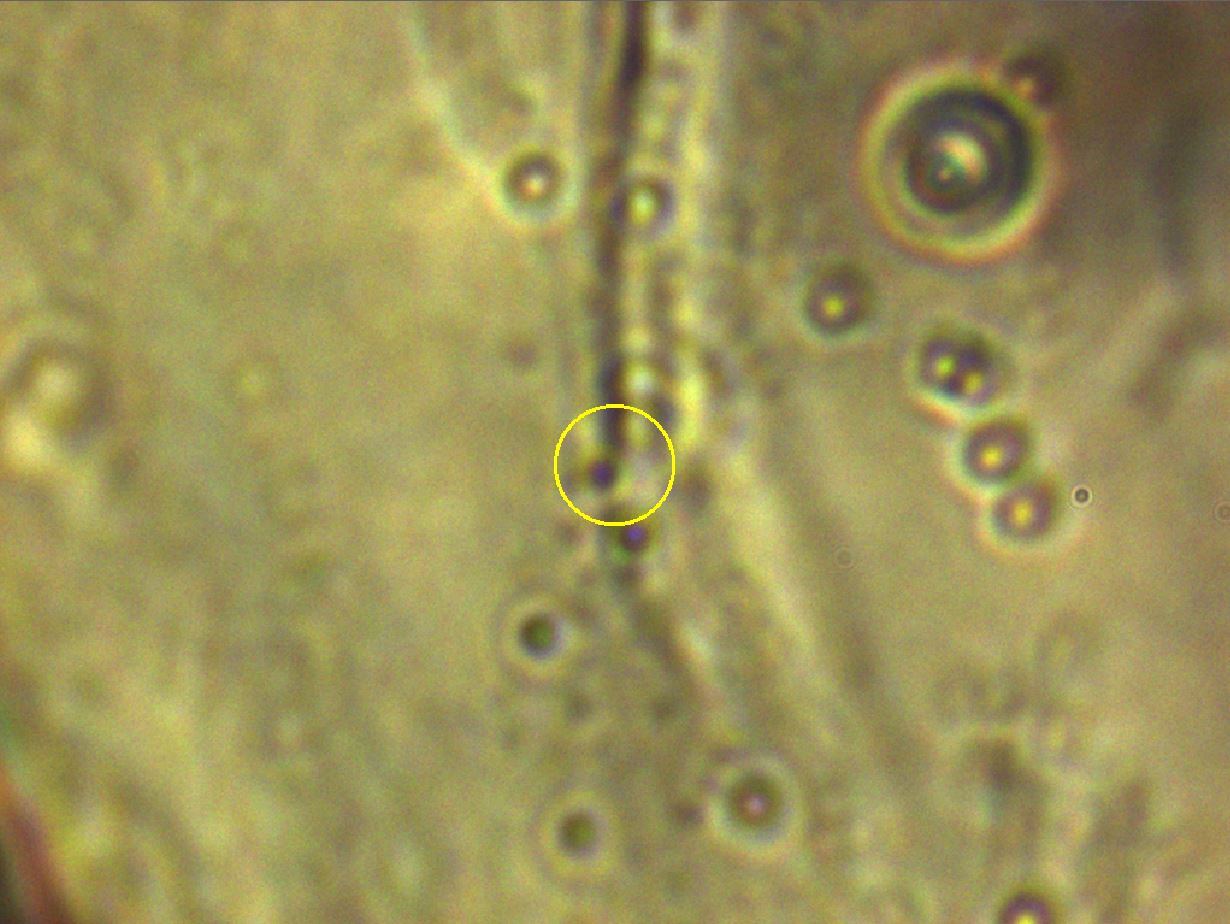
\includegraphics[width=0.5\textwidth]{bilder/Vesikel1.JPG}
        \caption{Mehrere Vesikel innerhalb einer Zwiebelzelle.}
        \label{fig:Vesikel1}
    \end{figure}
    \FloatBarrier
    Die Größe eines Vesikels wird mithilfe der schon bestimmten Pixelgröße in der Fokusebene festgestellt.
    Dafür wurde ein Vesikelpfad gefunden, wessen Vesikel sich in der Fokusebene bewegten.
    Das wurde erkannt, indem ein Vesikel dieses Pfades eingefangen wurde, welches daraufhin nicht größer oder kleiner wurde, also sich schon im Fokuspunkt der Falle befand.
    In \autoref{fig:Vesikel_Groesse} ist das Vesikel als blau umrandeter Kreis zu erkennen.
    Es hat einen Durchmesser von 112 Pixeln.
    Umgerechnet sind das ca. \qty{1.9}{\um}.
    \begin{figure}[ht]
        \centering\captionsetup{format=plain}
        \includegraphics[width=0.5\textwidth]{bilder/Vesikel_Größe.png}
        \caption{Blau umrandetes Vesikel, wessen Größe bestimmt wurde.}
        \label{fig:Vesikel_Groesse}
    \end{figure}
    \FloatBarrier
    Eine Auslenkung der Vesikel durch die optische Falle ist möglich.
    Die maximale Fallensteifigkeit, die mit den gegebenen Laserleistungen erreicht werden kann reicht jedoch nicht aus um sie komplett von der Aktin Faser zu trennen.
    Nach dem Freilassen der Vesikel kehren diese zu ihrer ursprünglichen Position zurück und setzen ihre Bewegung nach ca. \qty{1}{s} wieder in gleicher Richtung fort.
    Eine weitere Beobachtung die gemacht wurde ist, dass wenn ein Vesikel weit von seiner Aktin-Faser entfernt wurde, dass weitere Vesikel kurz an der Stelle der Auslenkung der Faser verlangsamt werden.

    Um die Geschwindigkeit der Vesikel zu bestimmen, wurde der Laser auf eine Aktin-Faser gerichtet.
    Dabei war die Laserleistung so stark reduziert, dass die Vesikel in ihrer Bewegung durch die Falle nicht eingeschränkt wurden.
    Das Diodensummensignal wurde abhängig von der Zeit aufgenommen, sodass aus der Dauer der Blockade des Laserlichtes durch das sich vorbei bewegende Vesikel seine Geschwindigkeit berechnet werden kann.
    In \autoref{fig:Vesikel_Geschwindigkeit} ist solch eine Messung dargestellt.
    Im grau hinterlegten Intervall von $\Delta t \approx \qty{0.15}{s}$ bewegt sich ein Vesikel durch den fokussierten Laserstrahl.
    \begin{figure}[ht]
        \centering\captionsetup{format=plain}
        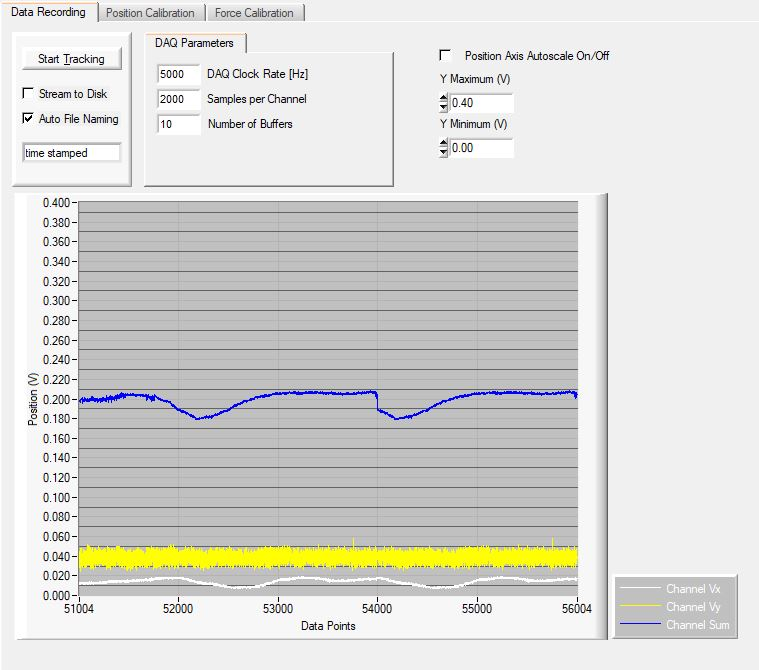
\includegraphics[width=0.6\textwidth]{plots/Vesikel_Geschwindigkeit.pdf} \vspace*{-0.5cm}
        \caption{Hier ist das Diodensummensignal gegen die Zeit aufgetragen, während zwei Vesikel hintereinander die Falle passieren.}
        \label{fig:Vesikel_Geschwindigkeit}
    \end{figure}
    \FloatBarrier

    Zur Bestimmung der Stärke der Aktin-Myosin-Motoren wurde die Falle auf einen Vesikelpfad fokussiert und die Laserleistung so weit hochgedreht, dass mindestens ein bewegtes Vesikel eingefangen wurde.
    Dies wurde für zehn verschiedene Vesikel wiederholt, sodass man einen Wert von $P \approx \qty{89.7}{mW}$ für die Grenzlaserleistung erhält, ab der die Vesikel eingefangen werden.
    Somit ergibt sich eine Grenz-Fallensteifigkeit von $k = \qty{7.63e-6}{N m^{-1}}$.
    

